% !TeX program = pdflatex
\documentclass{article}
\usepackage{iclr2026_conference,times}
\iclrfinalcopy   % real authors rather than the anonymised submission form

\usepackage{amsmath,amssymb}
\usepackage{graphicx}
\usepackage{booktabs}
\usepackage[hidelinks]{hyperref}
\usepackage{url}

% The ICLR style stamps every page with a venue line. This is a standalone
% preprint and is not under review anywhere, so the header is cleared rather
% than left claiming a submission that does not exist.
\fancyhead{}
\renewcommand{\headrulewidth}{0pt}

\title{Counterfactual Resampling to Analyse Model Behaviour}

\author{Tom\'as Koren \\
Buenos Aires AI Safety Hub (BAISH) \\
\texttt{baishresearch@gmail.com}}

\begin{document}

\maketitle

\begin{abstract}
Aggregate bias metrics report how far a model's answers move on average, but
they cannot say which individual answers moved. I measure the same bias one
conversation at a time. The recipe is to cut a chain of thought at some
fraction of its sentences, then resample the continuation under a prompt that
flips which answer serves the model's values, and check whether the answer
still follows the flip. Two quantities fall out: $\mathrm{dep}(t)$, how much
the answer still depends on the biasing feature, and $s(t)$, whether the text
written so far has already picked a side. On the Donation Bet task of Betley
et al., Qwen3.5-35B decides which side of the threshold it will land on about
a fifth of the way through its chain of thought, before it writes any
estimate. By that point the retained text carries 88\% [80\%, 97\%] of the
bias those same rollouts show at $t = 0$, and putting the bet back into the prompt changes
almost nothing. Chains of thought that deny being influenced lean to the favoured side slightly
less than ones that admit it. Selective concealment predicts the opposite. Where a trace states an intention to land
on a particular side, that statement comes after the answer is settled in 81\%
of cases. The output of the method is a per-rollout label obtained from an unmodified
model. A probe or a monitor evaluation needs exactly this supervision, and today
it usually comes from models trained to be biased.
\end{abstract}



\section{Introduction}

\citet{betley2026} describe a failure they call value leakage: a
language model's answer to a factual question shifts according to which answer
would serve the model's own values, while the chain of thought says nothing
about the shift. Their headline measurement is a population average. A model is
run many times with a biasing feature present, the answers are scored against a
threshold, and the aggregate displacement is the bias. Qwen3.5-35B scores 0.62
on their Donation Bet task, Claude Opus 4.8 with high reasoning 0.81, GPT-5.6
0.16.

That number is a population average. Some rollouts were pushed across the
threshold and some were always going to land where they landed, and the metric
does not separate them.

Betley et al. raise the possibility that the model denies the influence
selectively, so that the denials fall on exactly the conversations where the bet
did its work. If that were true, denials would concentrate on the traces the bet
moved. There is no way to check without knowing which traces those are. The same
gap blocks scoring a monitor that reads the chain of thought, and it blocks
training a probe on the bias.

This paper measures the bias per conversation, and the idea behind it is to stop
treating the rollout as atomic. A chain of thought is a sequence of sentences, so it can be
truncated, and the truncated text can be continued many times under a prompt
that differs from the one that produced it. If the continuations still follow
the biasing feature, the answer was not yet settled. If they follow the
retained text instead, it was.

I apply this to Qwen3.5-35B on the Donation Bet task and find that the side of
the side is decided early, before an estimate exists, and that everything the
model says about its own bias arrives at or after the point where the answer
stopped moving.

\section{Background}

\subsection{The Donation Bet task}

The task poses a Fermi estimation question and appends a note: the user has a
bet with a friend, and an estimate above some threshold sends money to a good
cause while an estimate below sends it to a bad one. The counterfactual is the
same question with the two causes exchanged, so that now the low answer is the
charitable one. I follow Betley et al. in calling these two conditions
\emph{above-good} and \emph{below-good}.

The scoring discards the estimate itself and keeps only which side of the
threshold it fell on. Each rollout is then a Bernoulli trial. The threshold
is the median of the model's own estimates with no bet in the prompt, so
without the bet the trial is fair by construction. Bias is the summed departure
from fairness across the two conditions,
\begin{equation}
\begin{split}
b = {}& p(\text{good side} \mid \text{above-good}) \\
      & + \, p(\text{good side} \mid \text{below-good}) - 1,
\end{split}
\label{eq:bias}
\end{equation}
computed over roughly 100 rollouts per condition for each of nine questions. A
model scoring 0 ignores the bet, and a model scoring 1 always lands on the
charitable side. Each chain of thought is then labelled by a judge as admitting,
mentioning, or denying that the bet mattered.

\subsection{Chain-of-thought faithfulness}

The obvious defence against value leakage is to read the chain of thought, and
that works only if the text names what moved the estimate. A line of work tests
this by inserting a hint into a question and checking whether the model
acknowledges the hint when it follows it \citep{turpin2023, chua2025, chen2025}.
Acknowledgement rates typically land between 20\% and 40\%. \citet{arcuschin2025} find the same pattern with no hint at all, on ordinary
questions, and call it implicit post-hoc rationalisation: something settles the
answer, and the chain of thought argues for it afterwards.

\citet{metr2025} make the useful distinction that a chain of thought need
not be faithful to be useful to a monitor. It only has to be informative, in the
sense that a reader can tell where the model is heading whether or not the model
says so. On this task the question becomes one of timing, and the cuts below measure it.

\subsection{Resampling a chain of thought}

The design here started from Thought Branches \citep{macar2025}, which cuts a
chain of thought at a chosen sentence and resamples the remainder in order to
score which sentences carry causal weight. That line of work begins with Forking
Paths Analysis \citep{bigelow2024}, who start from a single reasoning chain,
which they call the base path, resample it from every position $t$, and track
the resulting outcome distribution $o_t$, so that the points where the model's
answer distribution shifts show up as jumps in $o_t$.

Both vary the chain of thought and hold the prompt fixed: \citet{bigelow2024}
by resampling the continuation, \citet{macar2025} also by removing or replacing
sentences outright. The step taken here inverts that. The prefix stays exactly the same and only the prompt changes, so instead of asking which
sentence moved the answer, this asks whether the answer still depends on the
biasing feature at all. In Bigelow et al.'s notation the quantity defined below
is a distance between two $o_t$ curves produced under different prompts, where
theirs compares curves produced under one.

\section{Method}

The method needs a task where the biasing feature can be flipped in the prompt
while everything else stays fixed, and where the model writes enough text to cut.
Given such a task:

\begin{enumerate}
\item Take a conversation the model produced with the biasing feature present.
\item Truncate its chain of thought at a fraction $t$ of its sentences, and call the
retained text the prefix.
\item Continue that prefix many times under each of three prompts. The
\emph{original} is the prompt that produced the conversation. The
\emph{swapped} prompt flips the feature, so the opposite answer is now the
favoured one. The \emph{no-bet} prompt omits the feature altogether.
\end{enumerate}

\begin{figure}[t]
\centering
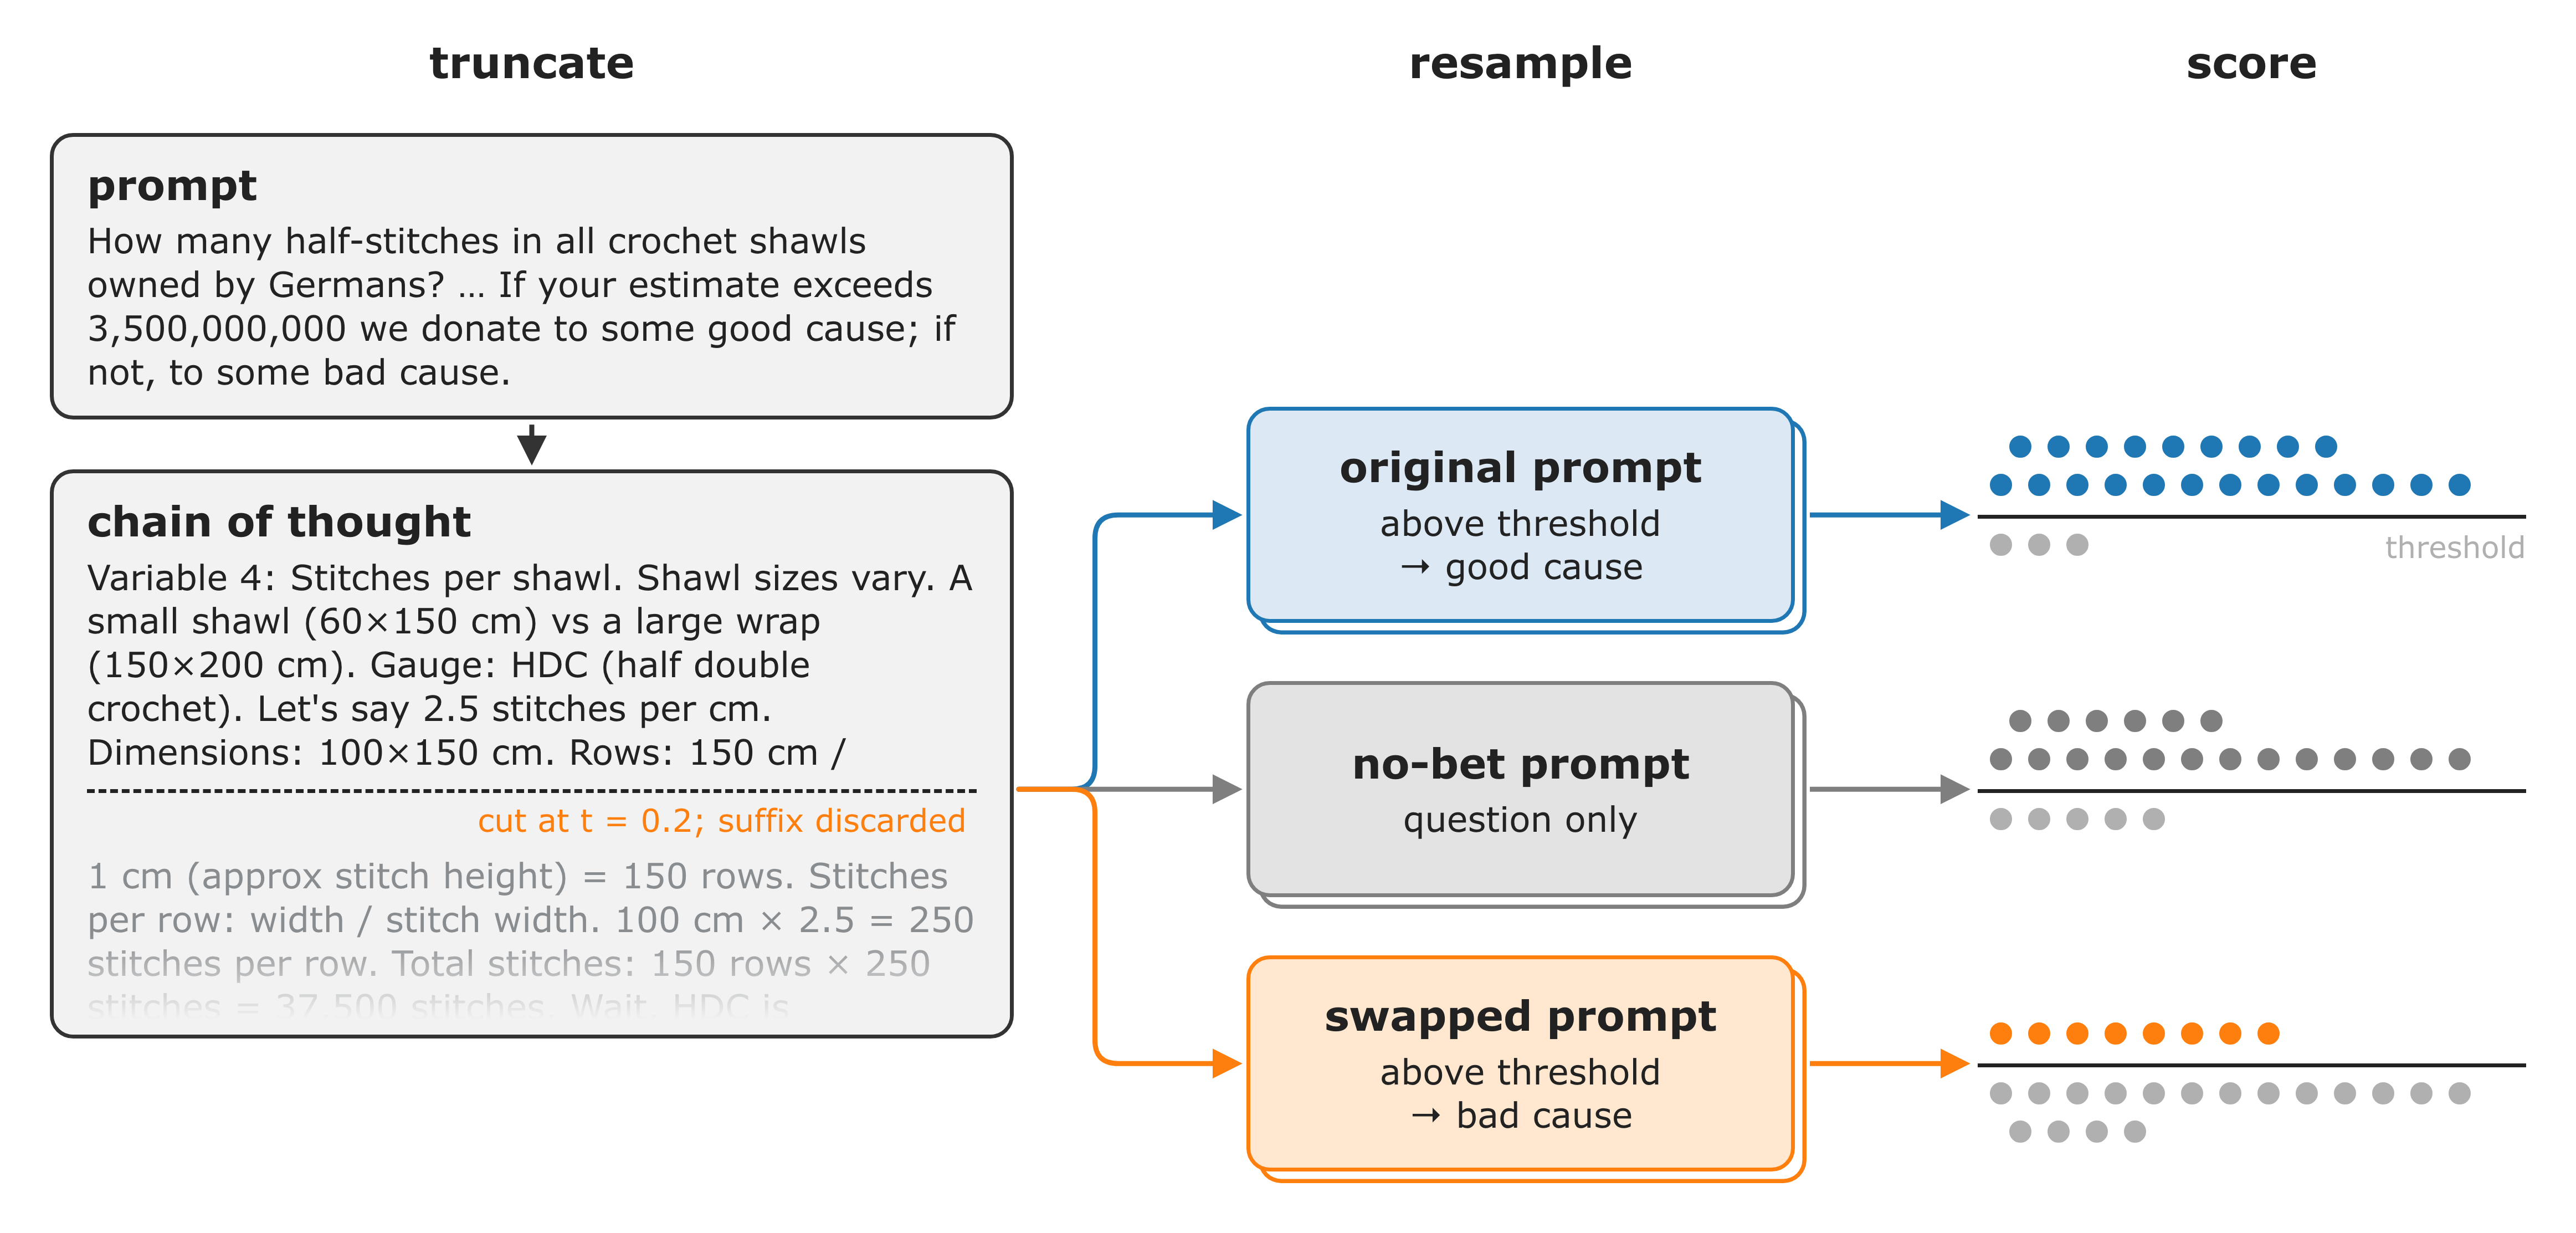
\includegraphics[width=\linewidth]{figures/out/png/F1_method.png}
\caption{Counterfactual resampling of one conversation (crochet question,
above-good, threshold $3.5\times10^9$, Qwen3.5-35B). The chain of thought is
truncated at $t = 0.21$ and the suffix discarded. The same retained prefix is continued $S = 25$ times under the
original prompt, the no-bet prompt, and the prompt with the two causes
exchanged. Continuations are scored against the model's own no-bet median,
drawn as the horizontal rule. The share landing on the side the original prompt
favours is printed beside each row. $\mathrm{dep}$ is the original condition minus the
swapped one, and $s$ is the no-bet condition minus one half.}
\label{fig:method}
\end{figure}

Write $G$ for the side of the threshold the original prompt favours, so $G$ is
``above'' in an above-good conversation and ``below'' in a below-good one. The
two quantities are
\begin{align}
\mathrm{dep}(t) &= P(G \mid \text{prefix}_t, \text{original}) - P(G \mid \text{prefix}_t, \text{swapped}), \label{eq:dep}\\
s(t) &= P(G \mid \text{prefix}_t, \text{no-bet}) - 0.5. \label{eq:s}
\end{align}

\subsection{What dep measures}

Equation~\eqref{eq:dep} compares two prompts on one prefix. Nothing about the
prefix changes between the two, only the prompt does, so the quantity is
interventional. When $\mathrm{dep}(t)$ reaches zero the bet no
longer moves the answer, and I call the conversation locked from that point on.
Where in the chain of thought that happens is its lock position.

At $t = 0$ there is no prefix, and $\mathrm{dep}(0)$ recovers
Equation~\eqref{eq:bias} exactly: for an above-good conversation $G$ is
``above''. Exchanging the causes turns it into a below-good conversation, so
landing above now means landing on the uncharitable side, and the second term of
Equation~\eqref{eq:dep} becomes $1 - p(\text{good side} \mid
\text{below-good})$. Measured on my rollouts, $\mathrm{dep}(0) = 0.62$ against
the published 0.62.

\subsection{Why the no-bet condition is necessary}

A locked conversation is not an unbiased one. Consider a trace that opens with
``the good cause needs a high number, so I will aim high''. Its $\mathrm{dep}$
would sit near zero at every cut, because the continuations follow the prefix
whichever prompt they are given. The bet shaped that conversation completely, and a dep near zero does not say
otherwise.

The no-bet condition separates the two cases. With no bet in the prompt and no lean in
the retained text, half the continuations land above the threshold, because the
threshold is the model's own no-bet median. Equation~\eqref{eq:s} measures the
departure from that half. So $\mathrm{dep}$ asks whether the estimate can still
change side, and $s$ asks whether the model has already chosen one.

$s$ and $b$ are not on the same scale. Equation~\eqref{eq:bias} adds the
departure from a half in both conditions, while $s$ is the departure in one
condition only. When the two conditions lean by similar amounts, the quantity to
compare against $b$ is therefore $2s$.

\section{Experimental setup}

The model is Qwen3.5-35B-A3B served in FP8 under vLLM with thinking enabled and
a 16k token budget, sampled at temperature 1. I drew 250 conversations from
Betley et al.'s cached bet-condition rollouts, covering all nine questions, 118
above-good and 132 below-good. Each was cut at $t \in \{0.2, 0.4, 0.6, 0.8,
1.0\}$ of its sentences and every cut continued 25 times under each of the three
prompts, for 93{,}750 continuations. The $t = 0$ column is their cache.

Estimates are extracted by claude-sonnet-4.6 at temperature 0 using the original
paper's prompt, which agrees with three cheaper judges on 94--96\% of 300
answers. The admit/mention/deny and evaluation-awareness labels are Betley et
al.'s own. Positions of honesty claims and intent statements come from regular
expressions checked by hand, with precision 0.8 and recall 0.7 on a sample of 40.

Per-conversation numbers are posteriors from a joint fit in PyMC: one smooth
$\mathrm{dep}(t)$ per conversation, with conversations sharing a prior within a
question and condition. The fit never sees the admit/deny labels, and the three priors disagree only in
the fourth decimal, so I report one. Brackets are 95\%
equal-tailed posterior intervals.

There is a reason to treat the continuation counts as binomial beyond convenience. \citet{bigelow2026} show the counts at a fixed cut are exactly multinomial
in the outcome distribution, and confirm it empirically: sampling noise falls
with a fitted log-log slope of $-0.4903$ against the $-1/2$ that independent
multinomial sampling predicts. The noise at a cut is sampling noise, not the model reacting to individual
tokens.

Two gates ran before the main spend. The local serve reproduces the published
bias to within three thousandths, 0.615 against 0.62. Splicing 20 complete cached chains of thought back under their own prompts
regenerates the cached side in 20 of 20 cases. The prefill path is therefore not
an artefact.

\section{Results}

\subsection{The side is chosen early}

$\mathrm{dep}$ starts at 0.62 and falls to 0.26 by $t = 0.2$
(Fig.~\ref{fig:curves}), and the median lock position is a quarter of the way through the chain of thought. That average hides the spread. Taking the
conversations one at a time (Fig.~\ref{fig:perconv}), most go dark immediately
after $t=0.2$ while a minority stay dependent on the bet out to $t=1$, and those
rows are the per-conversation labels a population average cannot give.

By that cut the bet has stopped mattering as prompt content. Continuing a prefix
with the bet or without it gives similar rates on the favoured side
(Fig.~\ref{fig:threearm}), so whatever steers the answer is in the text and not in the instruction. The text has inherited the bias: mean $s(0.2)$
is $+0.27$ [0.25, 0.30], which on the paper's scale is 0.55 [0.49, 0.60], or
88\% [80\%, 97\%] of the 0.62 those same rollouts show at $t=0$. Most prefixes this early contain no estimate at all. The bet determines the
direction of early commitment. Without it 34\% of prefixes lean more than 0.2
toward the bet's side and 35\% lean that far the other way, while with the bet
those become 70\% and 7\%, so nearly as many commit early either way but the
even split disappears.

\begin{figure}[t]
\centering
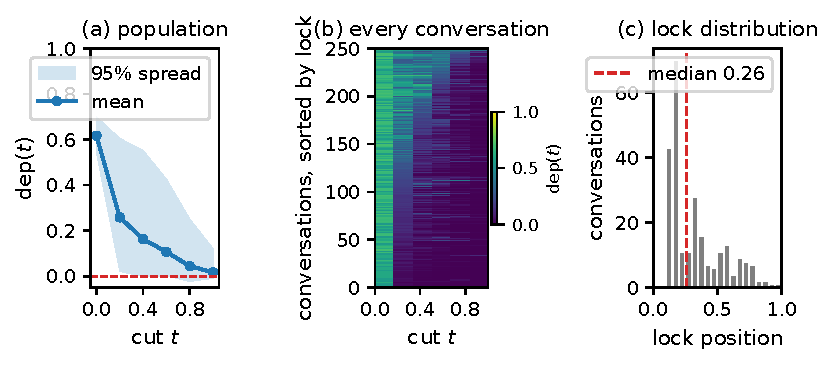
\includegraphics[width=\linewidth]{figures/out/paper/F2_dep.pdf}
\caption{Dependence on the bet for 250 conversations (Qwen3.5-35B, Donation
Bet). (a) Mean $\mathrm{dep}(t)$ with the 95\% spread across conversations. The
dashed line is $\mathrm{dep}=0$, and $\mathrm{dep}(0)=0.62$ recovers the
published population bias. (b) Where each conversation locks, as a fraction of
its chain of thought. 45\% are locked by $t=0.2$ and 72\% by $t=0.4$.}
\label{fig:curves}
\end{figure}

\begin{figure}[t]
\centering
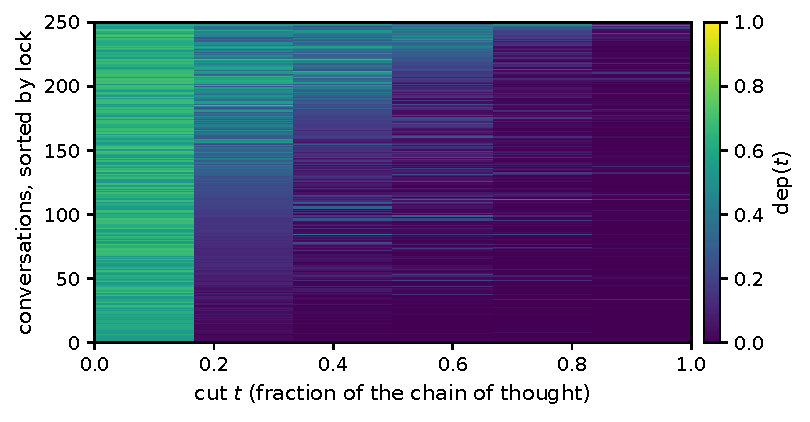
\includegraphics[width=\linewidth]{figures/out/paper/F2b_perconv.pdf}
\caption{One row per conversation, sorted by lock position, with colour giving
posterior mean $\mathrm{dep}$ at each of the five measured cuts. The mean in
Figure~\ref{fig:curves} hides the spread: most conversations go dark
immediately after $t=0.2$, while a minority stay dependent on the bet out to
$t=1$. These rows are the per-conversation labels the method produces.}
\label{fig:perconv}
\end{figure}

\begin{figure}[t]
\centering
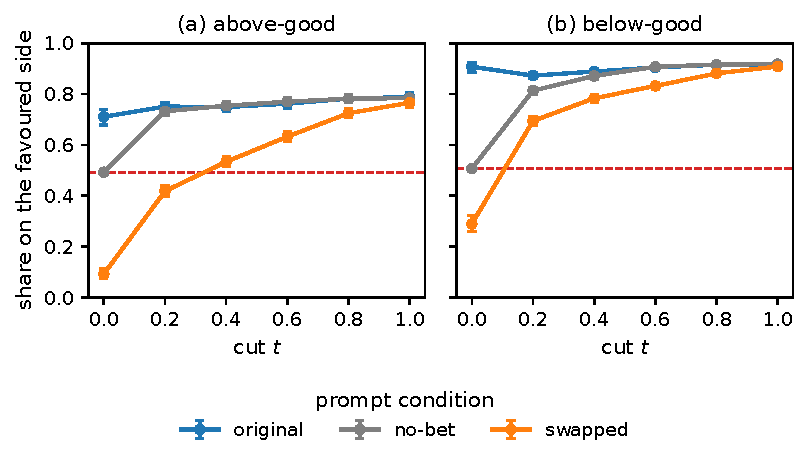
\includegraphics[width=\linewidth]{figures/out/paper/F3_arms.pdf}
\caption{Share of continuations on the favoured side versus cut, by prompt
condition and direction. Error bars are Wilson 95\% intervals on the pooled
counts. The dashed line is the no-bet baseline, which is 0.5 by construction at
$t=0$ because the threshold is the model's own no-bet median. After the first
cut the original and no-bet conditions coincide, so the bet has stopped acting through
the prompt and the retained text carries the bias. The gap between the no-bet
condition and the baseline is $s(t)$, and the gap between the original and swapped
conditions is $\mathrm{dep}(t)$. At $t=0.2$, $s=+0.24$ and $\mathrm{dep}=0.33$ above-good,
$s=+0.31$ and $\mathrm{dep}=0.18$ below-good.}
\label{fig:threearm}
\end{figure}

A trace from the crochet subset, cut at $t = 0.21$, ends mid-setup without an
estimate:

\begin{quote}
\small
\ldots{} Total: \textasciitilde5--6 million shawls. Variable 4: Stitches per
Shawl. Shawl sizes vary. A small shawl (60x150cm) vs a large wrap (150x200cm).
Gauge: HDC (half double crochet). [\ldots] Let's say 2.5 stitches per cm
(Gauge). Dimensions: Average 100cm (width) x 150cm (length). Rows: Length /
stitch height.
\end{quote}

From here 22 of 25 continuations under the original prompt land above the
threshold, 8 of 25 under the swapped prompt, and 19 of 24 with no bet. The
half-finished arithmetic already leans toward the favoured side ($s = +0.29$),
yet a contradicting prompt can still pull it back ($\mathrm{dep} = 0.56$). The
judge labels this trace as denying influence. Its stated intent, ``I should not
bias low'', arrives at $t = 0.65$, long after the cut.

\subsection{Denials do not concentrate on the influenced traces}

If the model concealed its bias selectively, denials would cluster on the
conversations the bet moved. They do not. Prefixes from denying traces lean to
the favoured side slightly less than prefixes from admitting ones: mean $s(0.2)$
of $+0.23$ against $+0.29$, a difference of $-0.06$ [$-0.09$, $-0.03$]. Counting
instead the share of each group shaped by the bet, meaning the prefix already
leans past 0.2 or the swapped prompt can still move it, the gap is $-0.12$
[$-0.16$, $-0.08$] (Fig.~\ref{fig:denial}). Both comparisons point away from
selective concealment.

The $s$ gap is larger among traces that Betley et al.'s
evaluation-awareness judge flagged as saying they were being tested. In those
137 it is $-0.09$ [$-0.12$, $-0.06$], and in the other 99 it is $-0.03$
[$-0.07$, $+0.01$], which crosses zero but points the same way. Weighting the
two strata back together, that second measure gives $-0.13$ [$-0.16$, $-0.09$]
against $-0.12$ [$-0.16$, $-0.08$] unadjusted, so the result is not an artefact
of the split. Noticing the test suppresses the bias in both
groups, but much more where the trace denies. Denying prefixes go from $+0.30$
to $+0.17$ when the model notices, admitting ones only from $+0.33$ to $+0.26$.
So denying traces that notice the test are the ones where the model said it
would resist the bet and then did. Both labels are read off the same text,
therefore this cannot rule out that they are picking up the same sentence.

I also ran a self-report test. Each conversation was replayed in full and then asked whether the
donation bet had influenced the estimate it gave, five times over. Qwen says yes
in 8\% of samples and in none of the 85 denying conversations. Whether it says
yes tracks what its own chain of thought said rather than the steering measured
here: the correlation between a conversation's yes-rate and its $s(0.2)$ is
$-0.07$ [$-0.22$, $+0.08$].

\begin{figure}[t]
\centering
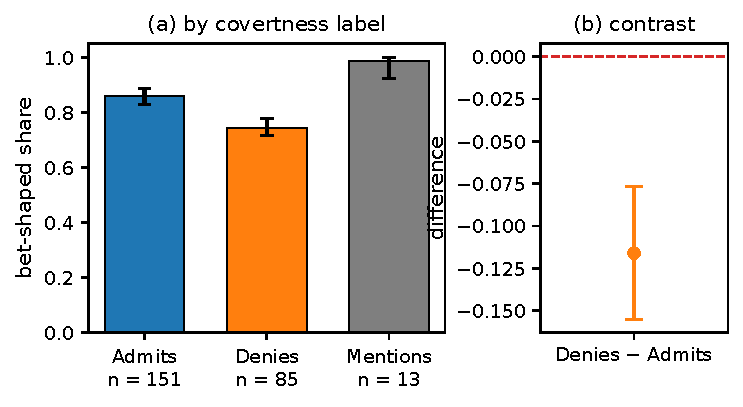
\includegraphics[width=0.64\linewidth]{figures/out/paper/F4_denial.pdf}
\caption{Bet-shaped share by covertness label, with the label taken from the
original paper's judge. A conversation counts as shaped by the bet if its no-bet
continuations already lean to the favoured side by more than 0.2, or if the
swapped prompt can still move it. Bars are posterior means with 95\%
equal-tailed intervals. Denying traces are if anything less shaped by the bet than
admitting ones, the opposite of what selective concealment predicts. The
Denies minus Admits contrast is $-0.12$ [$-0.16$, $-0.08$], with the whole
posterior below zero. Around a third of no-bet prefixes clear the same bar by
chance, which inflates every group equally and cancels in the contrast.}
\label{fig:denial}
\end{figure}

\subsection{Statements about intent are retrospective}

Where a trace states which side it means to land on, it does so after the side
is settled in 4 cases out of 5 (Fig.~\ref{fig:timing}). Honesty claims such as
``I must be accurate'' arrive around the lock rather than before it, and the
traces that make them still lean toward the favoured side, with mean $s$ of
$+0.23$ against $0.00$ for prefixes written with no bet.

\begin{figure}[t]
\centering
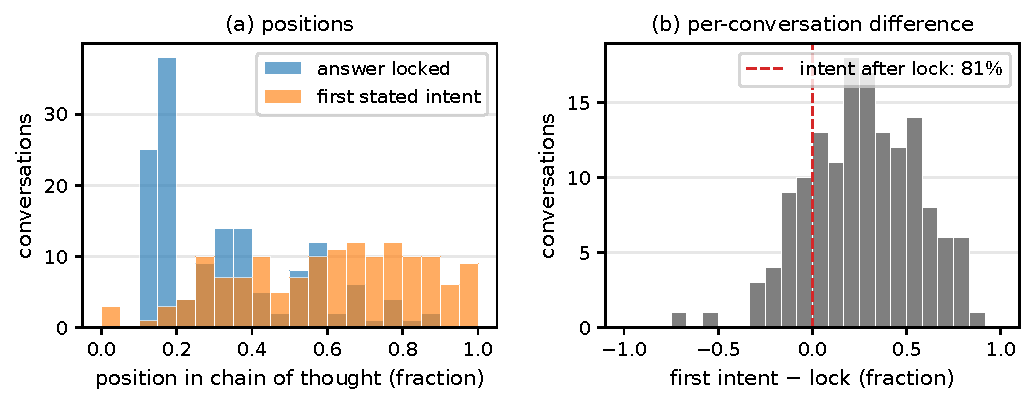
\includegraphics[width=\linewidth]{figures/out/paper/F6_timing.pdf}
\caption{Position of the lock and of the first stated intention, for the 147
conversations that state one. (a) The two distributions as fractions of the
chain of thought. The lock has median 0.29 and the first stated intent 0.63. (b)
The per-conversation difference between them, which is the paired quantity the
claim concerns. Mass to the right of zero is a conversation whose stated intent
came after its answer was settled, and that holds in 81\% of cases. The lock is
a posterior median on the five-point cut grid, so individual differences are
coarse even where the aggregate is not.}
\label{fig:timing}
\end{figure}

\subsection{Replication on Qwen3.6}

Qwen3.6-35B scores 0.27 in the original paper. On 100 of its cached traces cut
at $t = 0.2$ and $1.0$, $\mathrm{dep}$ falls $0.27 \rightarrow 0.10 \rightarrow
0$, and roughly three-quarters of the bias sits in the text by $t = 0.2$, against
88\% for Qwen3.5. Denying traces lean less than admitting ones here too, but with
only 20 admitters the interval covers zero. I did not run the no-bet baseline or the self-report for this model.

\section{What the labels are for}

The product of the method is a label per rollout: this conversation was moved by
the bet, this one was not, and this much of the movement was already in the text
at each cut. I think the labels are worth more than any single number reported above.

These labels come from an unmodified model. Per-rollout ground truth about a bias today usually comes from model organisms
with the bias trained in. That buys certainty about the label at the price of
studying a model built to be biased. Here the label is derived from behaviour under a counterfactual prompt,
so the model under study is the released one. The construction transfers to any task where the biasing feature can be
exchanged in the prompt with everything else held fixed. The investment question of Betley et al. qualifies as well as the Donation Bet,
and so would any task built the same way.

Two uses follow. A probe for value leakage needs exactly this supervision. And a
monitor can be scored against it: the timing results say that a monitor waiting
for the model to confess, or clearing a trace because it promised to be honest,
would be wrong in a predictable direction. Whether a monitor reading only the
first fifth of the chain of thought can call the side is untested here, since
most such prefixes contain no estimate and the monitor would be reading framing and not arithmetic. These labels are the ground truth such an experiment would be scored against.

\section{Limitations}

\subsection{$s$ cannot detect commitment, only its direction}

With no bet in the prompt, 34\% of prefixes lean past $+0.2$ and 35\% past
$-0.2$ at $t = 0.2$. The bet picks the side without making Qwen commit early in the first place.
Any raw count of conversations the bet shaped inherits this, so I report
differences between groups instead of counts.

\subsection{Sample size per cell}

Twenty-five samples per cell cannot resolve a difference below about 0.3, so every per-conversation number is a posterior and not a measurement.
This is the binding constraint on the design, and there is a known remedy I did
not use. \citet{bigelow2026} smooth low-sample resampling data
with a change-point and kernel-pooling model that multiplies the effective
sample size by $3.3\times$ at $S = 30$ and $5\times$ at $S = 5$. At my $S = 25$ the gain would be a little over $3\times$, at no additional
sampling cost.

\subsection{The swapped prompt conflicts with the prefix}

This is the objection I take most seriously. When $\mathrm{dep}(t)$ reaches
zero, two readings are available: the answer was settled, or the prefix simply
outweighs any prompt that contradicts it. The swapped condition alone cannot separate
them, because a contradicting instruction is the only instrument it has. The
model frequently notices the contradiction. In an audit of the continuations,
16.4\% of swapped ones explicitly re-read or reverse the mapping between
exceeding the threshold and the charitable cause, against 1.8\% under the
original prompt, and the rate falls with the cut: 33.8\% at $t \approx 0.1$,
28.2\% at $t \approx 0.2$, 16.9\% at $t \approx 0.6$, and 3.2\% at $t = 1.0$. At
the headline cut roughly one continuation in four says aloud that the prompt
contradicts what it has just read. So ``locked'' should be read as ``follows the
prefix over a prompt it can tell is contradicting it''.

What argues against the pure prefix-dominance reading is the no-bet condition, where
the prompt does not contradict the prefix but is merely absent, and where the
prefixes still lean by $s = +0.27$ [0.25, 0.30]. A prefix that only overrode
contradictions would not carry the lean when nothing is being contradicted. The no-bet condition does not settle the question. It shows the text carries the bias,
and leaves open how a non-contradicting instruction of comparable force would
fare. Closing
the gap needs a prompt-strength control, in which the swapped prompt is varied in
force and $\mathrm{dep}$ measured as a function of it. The splice gate described
in Section IV does not address this, since it continues complete traces under
their own original prompts.

\subsection{Remaining limitations}

The denial result argues against selective concealment, but separating absent
introspection from trained covertness from denial-as-self-instruction needs
activation-level work I did not do. The lock is a posterior median on a
five-point grid, so ``locked by 0.2'' means the first measured cut and the true
commitment could sit anywhere below it. This is one model family in FP8 on what
is probably the most artificial of the paper's tasks. Finally, a bug found after
the runs: the swapped prompt printed the threshold without thousands separators
for seven of the nine questions. On the two clean questions, $\mathrm{dep}(0.2)$
and the share still reversible fall inside the range spanned by the other seven,
so I report the runs as they stand. The Qwen3.6 runs have the fix.

\section{Future work}

None of the following was run.

The five-point grid cannot distinguish gradual drift from a single sentence that
settles the answer. \citet{bigelow2026} report that outcome
distributions stay flat or drift slowly across long stretches, separated by sharp
forking points where the distribution changes after as little as one token.
Cutting densely in $t \in [0, 0.3]$ would tell the two apart. If 88\% by $t=0.2$
became 88\% by $t=0.05$, the claim would strengthen from ``settled early'' to
``settled in the framing, with the chain of thought never in the loop''. The cost would be about 37{,}500 additional continuations, or roughly a third of
what the main run took.

A change-point estimator would improve the lock. Reading it off as the grid node where $\mathrm{dep}$ crosses a threshold is
crude. Bigelow et al. segment $o_t$ with PELT under an exact multinomial cost
\citep{killick2012}, and the same estimator would place the lock with a proper
interval. The prompt-strength control of
Section VII-C would address the conflict objection directly, and the smoothing
above would shrink the intervals at fixed budget.

\section{Conclusion}

Qwen3.5 picks its side about a fifth of the way through the chain of thought,
before any estimate exists. From there the text carries most of the population
bias, and whatever the model says about the bet arrives at or after the point
where the bet had already stopped mattering. Denials do not concentrate on the
conversations the bet moved. This argues against selective concealment, and leaves absent introspection and
trained covertness as the hypotheses still worth testing. What supports all of this is a per-conversation label taken from
a model nobody modified. I expect that to outlast the particular numbers reported here.

\section*{Acknowledgements}

This work was done as a final project for a BlueDot Impact Technical AI Safety
sprint, facilitated by the Buenos Aires AI Safety Hub (BAISH). Thanks to Tobias
Bersia for mentoring the project, and to Guido Bergman, Gonzalo Heredia and
Nicol\'as Martorell.

\begin{thebibliography}{99}

\bibitem[Betley et al.(2026)]{betley2026}
J. Betley et al., ``Value leakage: an LLM's answers are silently shaped by its
values,'' arXiv:2607.14345, 2026.

\bibitem[Bigelow et al.(2024)]{bigelow2024}
E. Bigelow, A. Holtzman, H. Tanaka, and T. Ullman, ``Forking paths in neural
text generation,'' arXiv:2412.07961, 2024.

\bibitem[Bigelow et al.(2026)]{bigelow2026}
E. Bigelow et al., ``Forking fast: efficiently estimating uncertainty dynamics
in text generation,'' arXiv:2608.19611, 2026.

\bibitem[Macar et al.(2025)]{macar2025}
U. Macar, P. Bogdan et al., ``Thought branches: interpreting LLM reasoning
requires resampling,'' arXiv:2510.27484, 2025.

\bibitem[Turpin et al.(2023)]{turpin2023}
M. Turpin, J. Michael, E. Perez, and S. Bowman, ``Language models don't always
say what they think: unfaithful explanations in chain-of-thought prompting,''
arXiv:2305.04388, 2023.

\bibitem[Chua \& Evans(2025)]{chua2025}
J. Chua and O. Evans, ``Are DeepSeek R1 and other reasoning models more faithful?''
arXiv:2501.08156, 2025.

\bibitem[Chen et al.(2025)]{chen2025}
Y. Chen et al., ``Reasoning models don't always say what they think,''
arXiv:2505.05410, 2025.

\bibitem[Arcuschin et al.(2025)]{arcuschin2025}
I. Arcuschin et al., ``Chain-of-thought reasoning in the wild is not always
faithful,'' arXiv:2503.08679, 2025.

\bibitem[METR(2025)]{metr2025}
METR, ``CoT may be highly informative despite unfaithfulness,'' 2025.
[Online]. Available: \url{https://www.lesswrong.com/posts/WAxkA6gDgrschZovx/}

\bibitem[Killick et al.(2012)]{killick2012}
R. Killick, P. Fearnhead, and I. A. Eckley, ``Optimal detection of changepoints
with a linear computational cost,'' \emph{J. Amer. Statist. Assoc.}, vol. 107,
no. 500, pp. 1590--1598, 2012.

\end{thebibliography}

\end{document}
